\section{Producing Francium}

This section is a collection of notes about how to go about making a source of
radioactive francium atoms, as needed for the project assembling FrAg
molecules---an entirely separate project and wholly irrelevant for \CENTREX.

\subsection{Isotope sources}

The longest-lived isotope, francium-223, can be obtained from the decay chain of
actinium-227 as shown in Fig.~\ref{Ac227}. In the following, we consider two
possible approaches to obtain a beam of francium, either an ion beam, or a
neutral atom beam. See also comparison in Table~\ref{ion_vs_neutral}.
\paragraph{Ion beam}

Following Guckert et al.\ \cite{guckert1998magneto},

\paragraph{Neutral atom beam}

\subsection{Safety considerations}

\begin{figure}
   \centering
  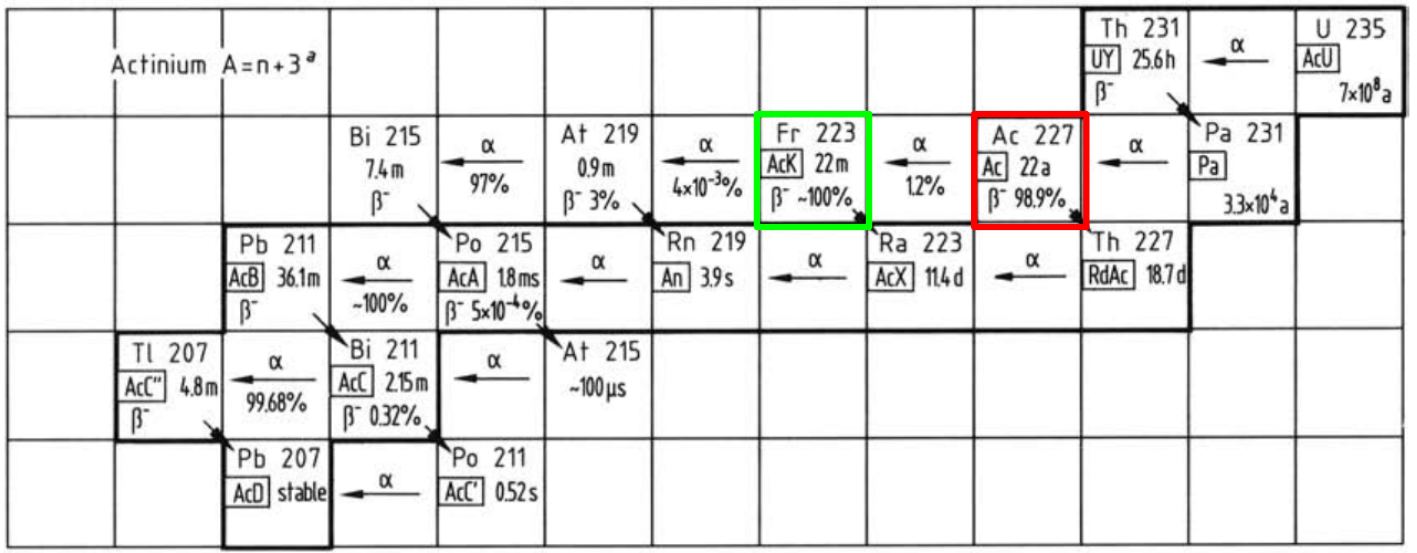
\includegraphics[width=\textwidth]{figs/todo/Ac227.png}
   \caption[Decay chain of actinium-227.]{Decay chain of actinium-227. Adapted from \cite{keller2000radionuclides}.}
  \label{Ac227}
\end{figure}

\begin{table*}
  %\small
  \makebox[\textwidth][c]{%
    \begin{tabu} to \textwidth {rcc}
      \toprule
                            & Ion beam                  & Neutral atom beam \\\midrule
       References           & \cite{guckert1998magneto} & \cite{dinneen1996orthotropic,lu1997efficient} \\
       Species              & Rb-82                     & Fr-221 \\
       Source activity      & 8 mCi                     & 9 $\mu$Ci \\
       Exit source          & 35 \%                     & 2 \% \\
       Enter cell           & 30 \%                     & 33 \% \\
       Trapping efficiency  & 0.3 \%                    & 56(10) \% \\
       Trap lifetime        & 30 s                      & 0.58(27) s \\
       \#\ of trapped atoms & $6\cdot10^6$              & $9\cdot10^2$ \\
      \bottomrule
    \end{tabu}}
    \caption{Comparing an ion beam to a neutral atom beam.}
    \label{ion_vs_neutral}
\end{table*}

